% Created 2020-04-07 周二 14:16
% Intended LaTeX compiler: pdflatex
\documentclass[11pt]{article}
\usepackage[utf8]{inputenc}
\usepackage[T1]{fontenc}
\usepackage{graphicx}
\usepackage{grffile}
\usepackage{longtable}
\usepackage{wrapfig}
\usepackage{rotating}
\usepackage[normalem]{ulem}
\usepackage{amsmath}
\usepackage{textcomp}
\usepackage{amssymb}
\usepackage{capt-of}
\usepackage{hyperref}
\usepackage[UTF8]{ctex}
\author{林韬}
\date{\today}
\title{Study of the online event filtering algorithm for BESIII 阅读笔记}
\hypersetup{
 pdfauthor={林韬},
 pdftitle={Study of the online event filtering algorithm for BESIII 阅读笔记},
 pdfkeywords={},
 pdfsubject={},
 pdfcreator={Emacs 26.3 (Org mode 9.3.6)}, 
 pdflang={English}}
\begin{document}

\maketitle
\tableofcontents

主要目标:
\begin{itemize}
\item 了解在线事例过滤算法如何处理一个巴巴事例 (Bhabha scattering events)
\end{itemize}

常见的几种事例类型
\begin{itemize}
\item 巴巴事例: e+e- -> e+e-
\item 缪子对产生:e+e- -> mu+mu-
\item 双光子:e+e- -> gamma gamma
\end{itemize}

Online filter system 主要作用
\begin{itemize}
\item 事例分类
\item 本底压低
\end{itemize}

EVT: event filtering software,是DAQ系统的一部分。

平均的时间延迟设计在 5ms。因此要求更快的处理器和算法。

在线过滤的框架部分采用 Step-by-step 技术,使用控制器配置和管理全局和局部的算法。

基于模拟数据进行事例的产生
\begin{itemize}
\item Bhlumi产生巴巴事例
\item radgg产生双光子事例
\item KKMC产生mu、tau、强子事例
\item EvtGen处理粒子的衰变
\end{itemize}

本底事例采用特别的产生子
\begin{itemize}
\item beam-gas样本
\item cosmic ray样本
\end{itemize}

一个在线处理的例子:

\begin{center}
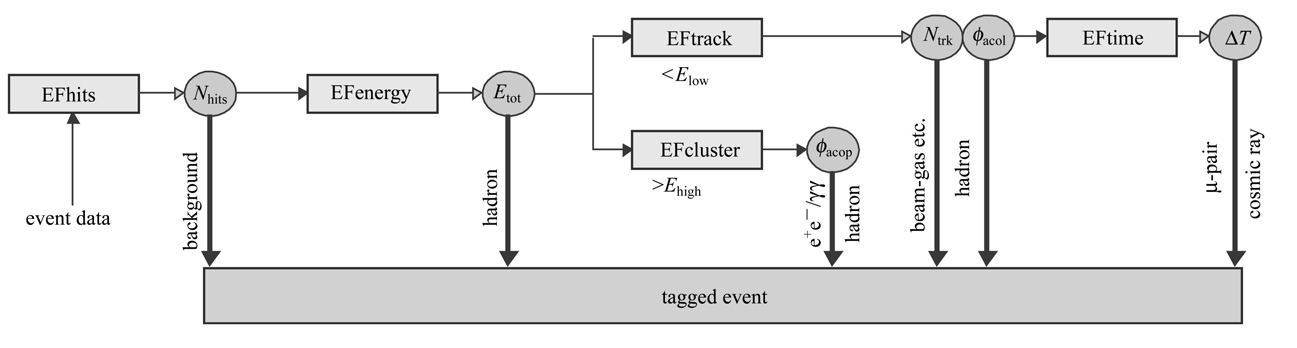
\includegraphics[width=.9\linewidth]{./figures/BESIIIFilterExample.png}
\end{center}


图中的方块表示算法,圆圈表示是后续算法用到的变量。

\begin{itemize}
\item N hits 小于 1000,信号。大于 1000,本底。
\item E tot in EMC
\begin{itemize}
\item 强子:在 Elow 和 Ehigh 之间
\item e+e-或gamma gamma:大于 E high
\item 其他待确定的类型:小于 Elow
\end{itemize}
\item Acoplanarity
\begin{itemize}
\item 巴巴事例和gamma gamma事例可以用于在线亮度的计算。
\item 但他们无法通过 EMC 的总沉积能量区分。
\item 在磁场作用下,带点粒子会发生偏转。因此可以通过重建shower位置来区分。
\item 定义 \(\cos\phi_{\mathrm{acop}} = -(\cos\varphi_1 \cos\varphi_2 + \sin\varphi_1 \sin\varphi_2)\)
\item 此处的 \(\varphi\) 是shower的方位角。
\item 所以上面的公式可以理解为两个矢量点乘。每个矢量的分量是 \(\cos\varphi\) 和 \$\(\sin \varphi\)\$。
\item 这样,该变量可以用于区分 e+e- 和 gamma gamma事例。
\item gamma gamma事例:小于 \(\phi_1\)
\item e+e-事例:在 \(\phi_2\) 和 \(\phi_3\) 之间
\end{itemize}
\end{itemize}
\end{document}
